% ============================================================================
% Chapter 3 — Results: Story A (paper-shaped unit)
% Pattern for all results chapters: chapter intro -> results -> summary.
% ============================================================================
\chapter{Results: [Title of Story A]}
\label{ch:resultsA}

\section{Introduction to this study}
\label{sec:resA-intro}
Brief chapter-specific background (1--2 pages) recapping only what this chapter
needs \citep{keyref2021}. Parts of this chapter are published: \citep{mypub2024}.

\section{Synthesis}
\label{sec:resA-synth}
\ldots{} Scheme~\ref{sch:3-1} summarises the route.

\begin{scheme}[htbp]
\centering
\schemestart
\chemfig{A-B}
\arrow{->[conditions][yield]}
\chemfig{C-D}
\schemestop
\caption{Synthetic route.}
\label{sch:3-1}
\end{scheme}

\section{Characterisation}
\label{sec:resA-char}
\ldots{} Figure~\ref{fig:3-1}. Crystallographic confirmation: compound \textbf{8}
crystallises in $P2_1/c$ \ldots{} (CCDC 2400001).

\begin{figure}[htbp]
\centering
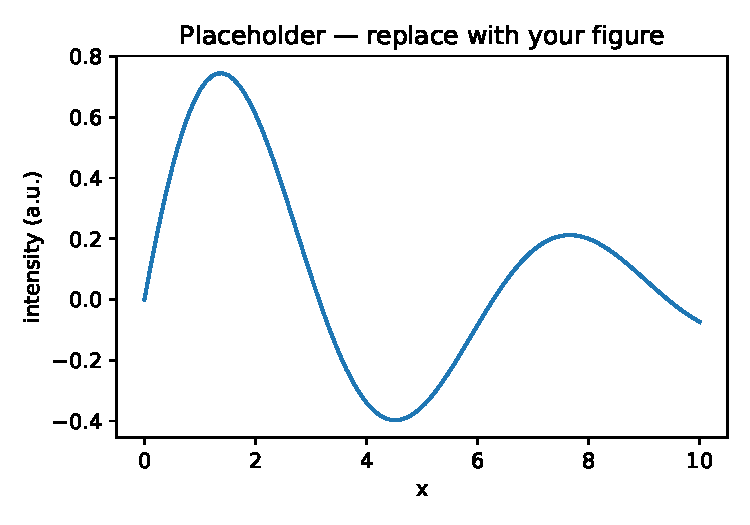
\includegraphics[width=0.8\linewidth]{fig31.pdf}
\caption{Key characterisation: X-ray structure / spectra / plot.}
\label{fig:3-1}
\end{figure}

\section{Discussion}
\label{sec:resA-disc}
\ldots{}

\section{Chapter summary}
\label{sec:resA-sum}
In this chapter, we demonstrated \ldots{} (3--5 sentences with data).
